\documentclass[]{article}
\usepackage{amsmath}\usepackage{amsfonts}
\usepackage[margin=1in,footskip=0.25in]{geometry}
\usepackage{mathtools}
\usepackage{hyperref}
\hypersetup{
    colorlinks=true,
    linkcolor=blue,
    filecolor=magenta,
    urlcolor=cyan,
}
\usepackage[final]{graphicx}
\usepackage{listings}
\usepackage{courier}
\lstset{basicstyle=\footnotesize\ttfamily,breaklines=true}
\newcommand{\indep}{\perp \!\!\! \perp}
% \usepackage{wrapfig}
\graphicspath{{.}}
% \usepackage{fancyvrb}

%%
%% Julia definition (c) 2014 Jubobs
%%
\usepackage[T1]{fontenc}
\usepackage{beramono}
\usepackage[usenames,dvipsnames]{xcolor}
\lstdefinelanguage{Julia}%
  {morekeywords={abstract,break,case,catch,const,continue,do,else,elseif,%
      end,export,false,for,function,immutable,import,importall,if,in,%
      macro,module,otherwise,quote,return,switch,true,try,type,typealias,%
      using,while},%
   sensitive=true,%
   alsoother={$},%
   morecomment=[l]\#,%
   morecomment=[n]{\#=}{=\#},%
   morestring=[s]{"}{"},%
   morestring=[m]{'}{'},%
}[keywords,comments,strings]%



% \lstset{%
%     language         = Julia,
%     basicstyle       = \ttfamily,
%     keywordstyle     = \bfseries\color{blue},
%     stringstyle      = \color{magenta},
%     commentstyle     = \color{ForestGreen},
%     showstringspaces = false,
% }
\begin{document}
\begin{center}
    Name: Hongda Li
    \\
    AMATH 585 WINTER 2022 HW 6
\end{center}
\section*{Problem 1}
    Any function with chebyshev coefficients $a_0, a_1, \cdots, a_n$, evaluated at the chbyshev node is given as: 
    \begin{align*}\tag{1}\label{eqn:1}
        p(\cos(k\pi/n)) &= 
        \sum_{j = 0}^{n}a_j\cos(jk\pi/n)
    \end{align*}
    Our objective here is make use hf the FFT algorithm for DFT for the objective of: Interpolation the function at chebyshev node getting the values of $a_0, a_1, \cdots, a_n$, and evaluating the function value at the chebyshev nodes using the FFT algorithm. It's implied that $k, n$ are integers in this context. 
    \par
    My claim here is that, if we tiled the vector in the following format:
    $$\vec{f} = [a_0, a_1, \cdots, a_{n - 1}, a_n, a_{n - 1}, \cdots, a_1]$$
    It's symmetric exclusing the first element, and then we put this into the DFT algorithm using FFT, then we obtain the following relationsship: 
    \begin{align*}\tag{1.1}\label{eqn:1.1}
        \frac{1}{2}(F_k + a_0 + (-1)^k)
        &= 
        \sum_{j = 0}^{n}\cos\left(
            \frac{\pi j k}{n}
        \right)a_j \quad \forall 0 \le k \le n
    \end{align*}
    Here, we assume that the vector $\vec{F} = [F_0, F_1, \cdots F_{2n - 1}]$ are the output of the DFT after we feed $\vec{f}$ into the algorithm. 
    \par
    Before we prove \hyperref[eqn:1.1]{(1.1)} we wish to establish some basics about the vector $\vec{f}$. Observe that the vector is symmetric if we exclude the first argument, which means that $f_j = f_{2n - j}\; \forall\; 1 \le j \le 2n - 1$. Next, the vector $\vec{f}$ has a total length of $2n$. And when we index the vector $\vec{f}, \vec{F}$, we let the \textbf{index starts with zero}. 
    \par
    First, consider the following algebra: 
    \begin{align*}\tag{1.2}\label{eqn:1.2}
        \exp\left(
            -i\frac{\pi(2n - j)k}{n}
        \right) &= 
        \exp\left(
            -i \frac{2\pi n - j\pi k}{n}
        \right)
        \\
        &= \exp
        \left(
            -i\frac{2n\pi n}{n} + \frac{ij\pi k}{n}
        \right)
        \\
        &= \exp\left(
            i\frac{jk\pi}{n}
        \right)
        \\
        \sum_{j = 0}^{2n - 1}
        \exp\left(
            -i \frac{i\pi j k}{n}
        \right) &= 
        \sum_{j = 1}^{2n}
        \exp\left(
            -i \frac{2\pi(2n - j)k}{n}
        \right)
    \end{align*}
    The second equality is just a trick where I swapp the index so it starts summing in the reverse order. 
    \par
    Now consider the DFT on vector $\vec{f}$, which by definition would be given as: 
    \begin{align*}\tag{1.3}\label{eqn:1.3}
        F_k &= \sum_{j = 0}^{2n - 1}
            \exp\left(
                - i \frac{2\pi j k}{2n}
            \right)f_j
        = \sum_{j = 0}^{2n - 1}
        \exp\left(
            - i \frac{\pi j k}{n}
        \right)f_j
        \\
        &= 
        \frac{1}{2}
        \left(
            \sum_{j = 0}^{2n - 1}
            \exp
            \left(
                -i\frac{\pi j k}{n}
            \right)f_j
            + 
            \sum_{j = 1}^{2n}
            \exp\left(
                -i \frac{2\pi (2n - j)k}{n}
            \right)\underbrace{f_{2n -j}}_{= f_j}
        \right)
        \\
        &= 
        \frac{1}{2}
        \left(
            \sum_{j = 0}^{2n - 1}
            \exp
            \left(
                -i\frac{\pi j k}{n}
            \right)f_j
            + 
            \sum_{j = 1}^{2n}
            \exp\left(
                i\frac{jk\pi}{n}
            \right)f_j
        \right) \impliedby \quad \text{by: \hyperref[eqn:1.2]{(1.2)}}
        \\
        &= \frac{1}{2}
        \left(
            2f_0 + 
            \sum_{j = 1}^{2n - 1}
            \exp
            \left(
                -i\frac{\pi j k}{n}
            \right)f_j
            + 
            \sum_{j = 1}^{2n - 1}
            \exp\left(
                i\frac{jk\pi}{n}
            \right)f_j
        \right)
        \\
        &= f_0 + \sum_{j = 1}^{2n - 1}
        \cos\left(
            \frac{\pi j k}{n}
        \right)f_j
    \end{align*}
    Next, please observe the fact that the term for $j = 1$ equals to $j = 2n - 1$, due to the symmetry of $\cos$ and the symmetry of vector $f_j\; \forall 1 \le j \le 2n - 1$. And hence we obtained: 
    \begin{align*}\tag{1.4}\label{eqn:1.4}
        F_k &= a_0 + \left(
            2 \sum_{j = 1}^{n - 1}
            \cos\left(
                \frac{\pi j k}{n}
            \right)a_j
        \right) + (-1)^k a_n
    \end{align*}    
    Here, take note of the extra term, when $j = n$, $f_j = n$, which is right in the middle of the symmetric part of $\vec{f}$, and it only repeats once, so I take it out from the sum and it produces the term $(- 1)^ka_n$. All other terms repeats 2 times and $f_0 = a_0$. Rearranging the above equation we have: 
    \begin{align*}\tag{1.5}\label{eqn:1.5}
        \frac{1}{2}
        \left(
            F_k - a_0 - (-1)^ka_n
        \right) &= 
        \sum_{j = 1}^{n - 1}
        \cos \left(
            \frac{\pi j k}{n}
        \right)a_j
        \\
        \frac{1}{2}
        \left(
            F_k + a_0 + (-1)^ka_n
        \right) &= 
        \sum_{j = 0}^{n}
        \cos \left(
            \frac{\pi j k}{n}
        \right)a_j
        \\
        \frac{1}{2}
        \left(
            F_k + a_0 + (-1)^ka_n
        \right) &= p\left(
            \cos\left(
                \frac{k\pi}{n}
            \right)
        \right)
    \end{align*}
    From the frist line to the second line, I added $a_0, (-1)^ka_n$ to both side of the equation. At this point, we have proven that \hyperref[eqn:1.1]{(1.1)} is true, and we can make use of the algorithm fast evaluate the chebyshev series at the chebyshev nodes. Simply make the vector $\vec{f}$ as said above, and then evalute it to get $F_k$, and then use that above expression, for $k = 0, \cdots, n$. There will be $2n$ output vectors, but we can ignore the part where it gets symmetric. 
    \par
    Next, to reverse the process for looking for the chebyshee coefficients, we simply consider: "What is $F_k$"? And then make use of the IDFT algorithm which uses IFFT. 
    \begin{align*}\tag{1.6}\label{eqn:1.6}
        p\left(
            \cos\left(
                \frac{k\pi}{n}
            \right)
        \right) &= 
        \frac{1}{2}
        \left(
            F_k + a_0 + (-1)^ka_n
        \right)
        \\
        2 p\left(
            \cos \left(
                \frac{k\pi }{n}
            \right)
        \right)  
        &= F_k + a_0 + (-1)^ka_n
        \\
        2 p\left(
            \cos \left(
                \frac{k\pi }{n}
            \right)
        \right) - a_0 - (-1)^ka_n
        &= F_k
    \end{align*}
    Do this for $k = 0, \cdots, 2n - 1$ and then invoke the IFDT using FFT, and then we get back the veoctr $\vec{f}$, and the first $n + 1$ elements are the chbyshev coefficients. 

\section*{Problem 2}
    \subsection*{Code}
    \lstinputlisting[language=matlab]{steady2d.m}
    \lstinputlisting[language=matlab]{MakeTestProblem.m}
    \lstinputlisting[language=matlab]{StationaryIterative.m}
    Error for all methods are measured using the relative error of the residual, which is given as $\Vert Ax_k -b\Vert/\Vert b\Vert$, and it's put under $\log10$. All methods tolerance are set to be $10^{-8}$ with zero vector as the initial guess. 
    \par
    Results are produced. This is a plot of the convergence of the errors for Staionary Iterative Methods: ``JB, GS, SOR'': 
    \begin{center}
        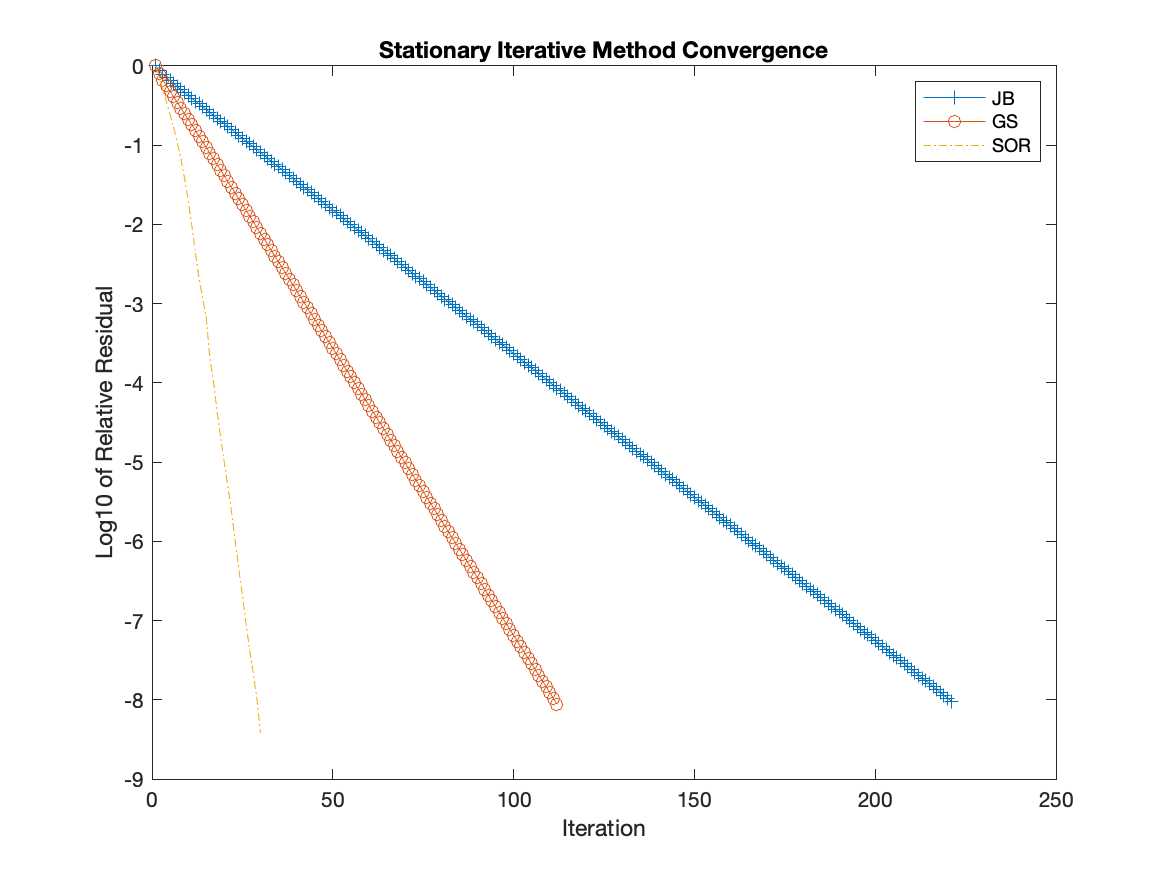
\includegraphics[width=10cm]{stationary_methods.png}
    \end{center}
    \par
    I computed the relexation factor using the maximal absolute eigen value of the Jacobi Split matrix: $-D^{-1}(L +U)$. And then I used the formula: $\omega_{\text{opt}} = \frac{2}{1 + \sqrt{1 - \rho(G_j)^2}}$, which gives the fastest descend of the error. 

    \begin{center}
        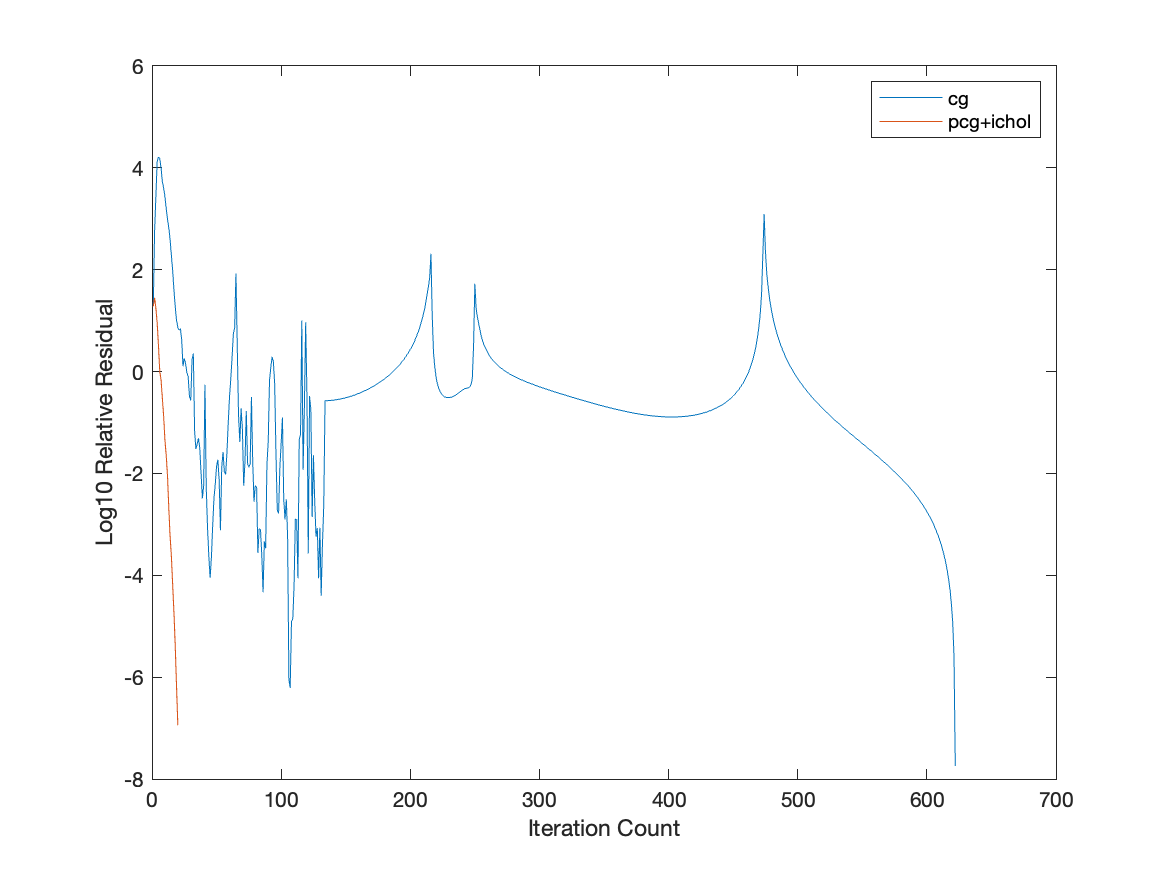
\includegraphics[width=10cm]{pcg_vs_cgs_itr.png}
    \end{center}
    \par
    This is the error of the Conjugate Gradient with and without preconditioneer. For the Preconditioner, we use Incomplete Cholesky Factorization. Observe that the relative residual is not monotonically decreasing for CG, because CG aims for minization on the energy norm induces by matrix $A$, and the relative residual error is not measured under that norm, therefore, it looks wacky like that. 
    \begin{center}
        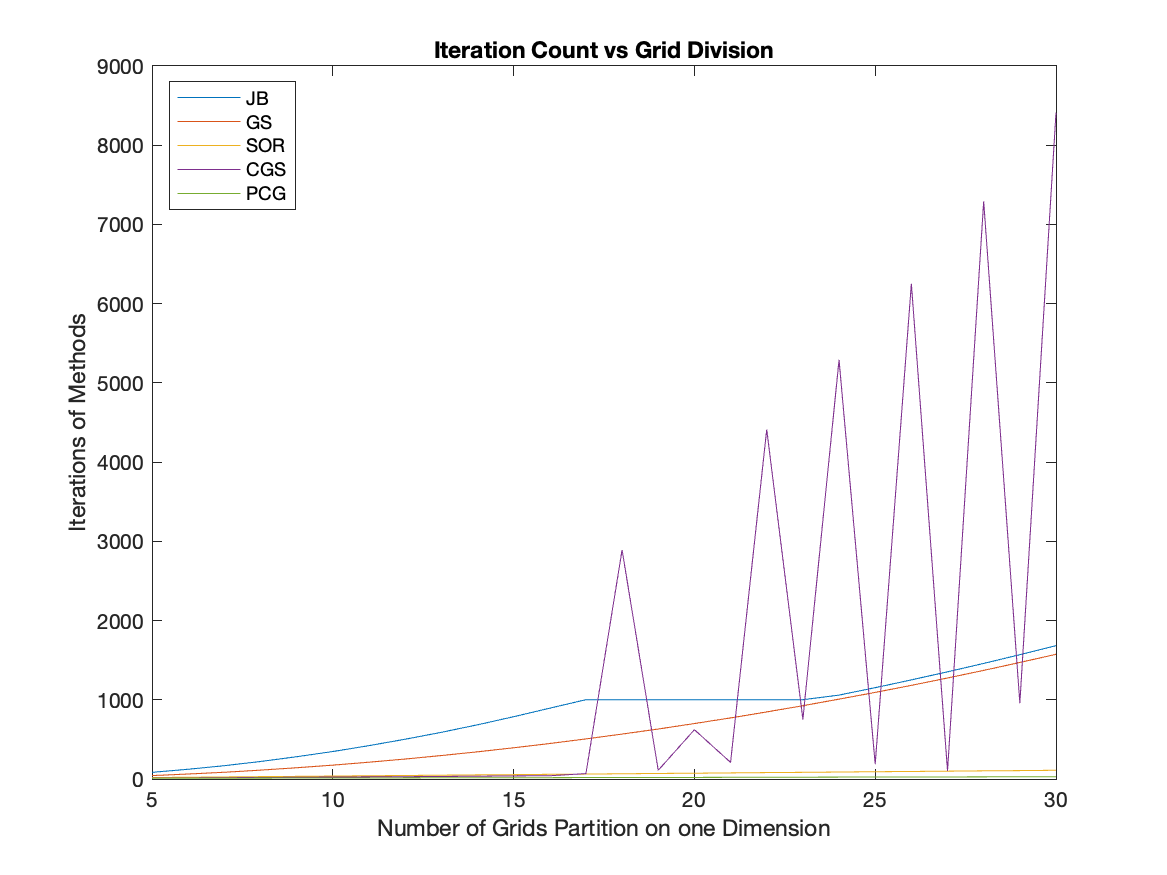
\includegraphics[width=10cm]{h_vs_methods_itr.png}
    \end{center}
    This is a plot of all methods iterations count versus the number of division along one dimension of the grid: $m$, which is basically $1/h$. 
    \par
    Please observe that, there are wilde oscilations (I don't know why) on the Conjugate Gradient methods, but the over all tenency grows quadratically. This is expected becaue the matrix is $m^2\times m^2$ where $m$ is the number of divisions along one dimension, and we know CG converges in the $n$ steps for a $n\times n$ matrix. 
    \begin{center}
        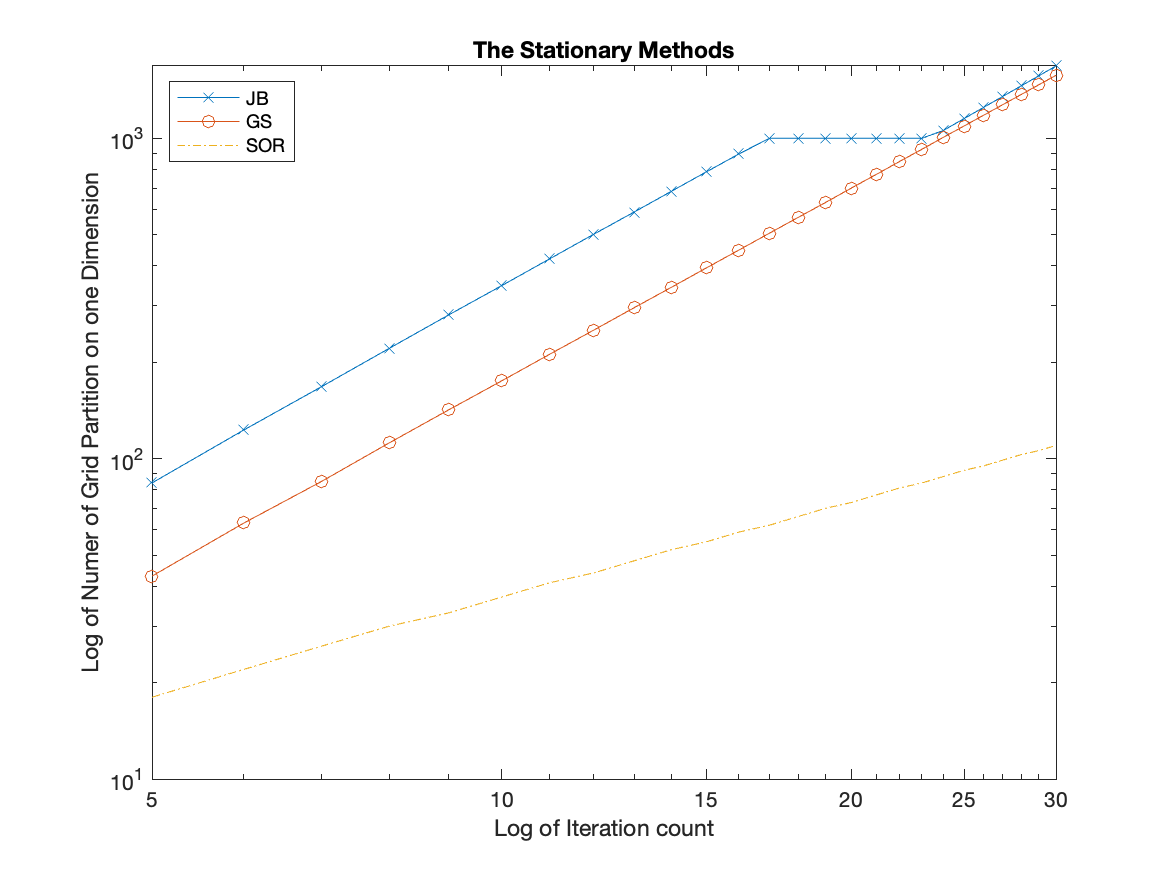
\includegraphics[width=10cm]{h_vs_stationary_methods.png}
        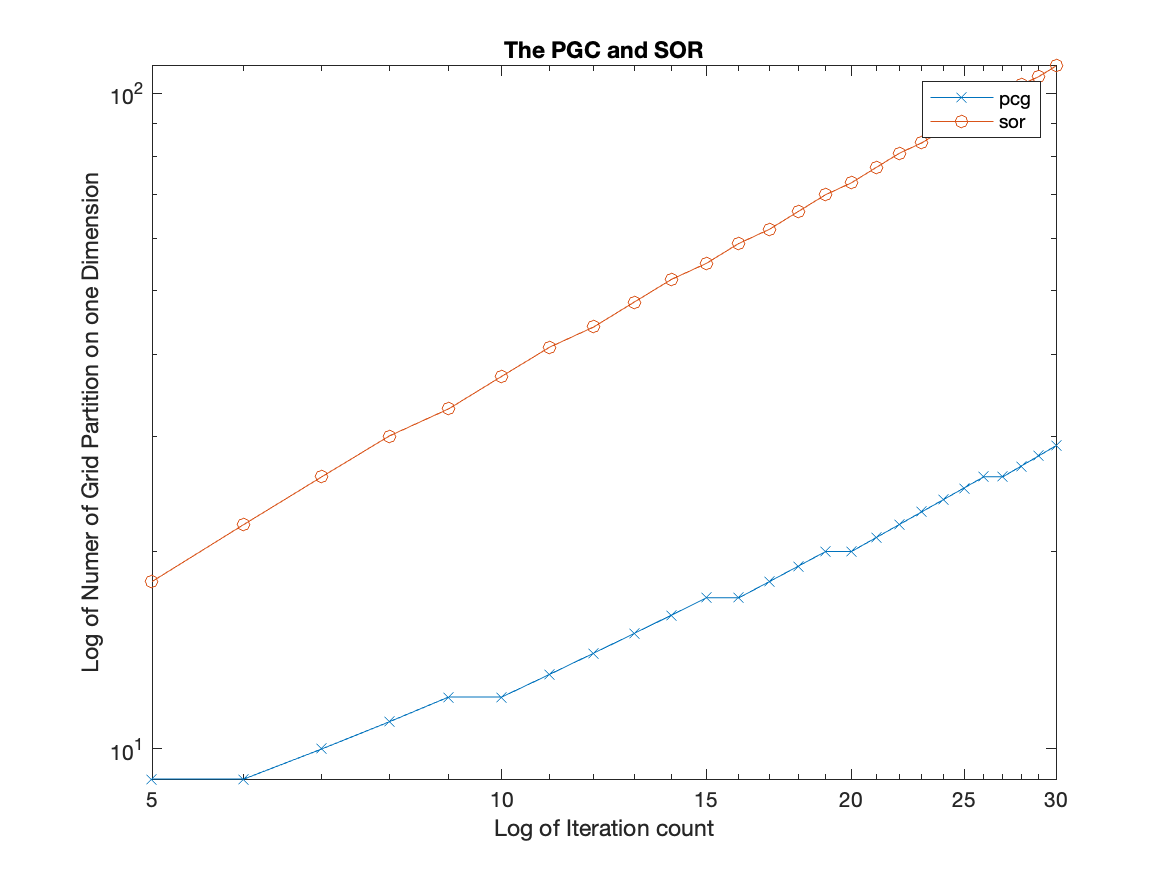
\includegraphics[width=10cm]{h_vs_pcg_sor.png}    
    \end{center}
    For further investigation, I plotted out the loglog of iteration count against the number of division along one axis. I computed the slope under the log log plot and obtained: 
    \begin{enumerate}
        \item [1.]SOR: 1.0259
        \item [2.]GS: 2.0179
        \item [3.]PCG: 0.5556
    \end{enumerate}
    I can explain the first 2, but the third one is one information for me. The SOR is expected to have this relation because how the spectrum of the iteration matrix, denoted by $\rho(G_{\text{sor}}) = 1 - \mathcal{O}(h)$, and for GS, the spectrum of the iteration matrix $\rho(G_{GS})= 1 -\mathcal{O}(h^2)$. And this is the reason why the above plot is observed. However, this doesn't mean that PC is necessary faster than all methods, because the Implete Cholesky is already an at least $O(m^2)$ cost. But it's obvious that CGS doesn't work well consistently, and it's on the same ballmark compare to GS and JB. 
    \par
    Here is a short justification for how SOR method has this relation between log of iteration cout and the log of number of discretizations along one dimension. Let $n$ denotes the number of iterations, $h$ denotes the width of the grid, and $h = 1/m$, and $\epsilon$ denotes the tolerance of the method. 
    \begin{align*}\tag{2.1}\label{eqn:2.1}
        (1 - \mathcal{O}(h))^n &< \epsilon
        \\
        1 - n\mathcal{O}(h) &<  \epsilon
        \\
        1 + \epsilon &< n\mathcal{O}(h)
        \\
        \frac{1 - \epsilon}{\mathcal{O}(h)} < n
        \\
        \implies n \propto m \propto \frac{1}{n}
    \end{align*}
    This implies a linear relations between the number of grid discritizations and the number of steps required for the SOR method to converge on a fixed tolerance. It's expected to be a linear function, which matches with our experiement. A similar relations can also be derived for the GS method, and we will get back a quadratic relations. 
    
\section*{Problem 3}
    Let's state the theorem for the convergence of the Conjugate Gradient Method in the following way: 
    $$
    \frac{\Vert e^{(k)}\Vert_A}{\Vert e^{(0)}\Vert_A} \le 
    \min_{p_k: p_k(0) = 1}\max_{x\in [\lambda_{\text{min}}, \lambda_{\text{max}}]} |p_k(x)|
    $$
    And the theorem that help us with a bound over the whole interval $[\lambda_{\min},\lambda_{\max}]$ is to use the Chebyshev Polynomial. The chebyshev is not the best bound, but it will help us to derive an upper bound, and repurpose it to the whole interval. 
    \begin{align*}\tag{3.1}\label{eqn:3.1}
        p_k(x) = \frac{T_k(\varphi(x))}{T_k(\varphi(0))}
        \quad \varphi(x) = \frac{2x - \lambda_1 - \lambda_n}{\lambda_n - \lambda_1}
    \end{align*}
    We repurpose the Chebesheve Polynomial and adapted it fit the optimal polynomial that bound the relative error of energy norm. Obesrve that when $x = 0$, it outputs one. And Chebeyshev polynomial has this inf norm minimizing quality that minimizes the polynomial over the spectrum of matrix $A$. 
    \par
    Finally, the theorem we derived during class is a bound on such polynomial, which is given as: 
    \begin{align*}\tag{3.2}\label{eqn:3.2} 
        \min_{p_k: p_k(0) = 1}\max_{x\in [\lambda_{\text{min}}, \lambda_{\text{max}}]} |p_k(x)| 
        \le
        \max_{x\in[\lambda_{\min}, \lambda_{\max}]}
        \left|
            \frac{T_k(\varphi(x))}{T_k(\varphi(0))} 
        \right|
        \le
        2 \left(
        \frac{\sqrt{\kappa} + 1}{\sqrt{\kappa} - 1}
        \right)^k
    \end{align*}
    Suppose that, the matrix $A$ has $n - 1$ eigenvalues that are very close to the origin and one eigenvalue $\lambda_n$ that are extremely huge compare to the other eigenvalues, then we consider a the product of the chebyshev polynomial with a linear interpolant that passes through the large eigenvalue. 
    \begin{align*}\tag{3.3}\label{eqn:3.3}
        p_k(z) &= 
        \frac
        {
            T_{k-1}\left(
                \frac{2z - \lambda_{n-1} - \lambda_1}{\lambda_{n-1} -\lambda_n}
            \right)
        }{
            T_{k-1}\left(
                \frac{
                    -\lambda_{n-1} - \lambda_1
                }
                {
                    \lambda_{n-1} - \lambda_1
                }
            \right)
        }\frac{\lambda_n - z}{\lambda_n}
        \\
        \hat{T}_{[a, b]}^{(k)}(x) &:= 
        T_k\left(
            \frac{2x - b - a}{b - a}
        \right) \leftarrow \text{For notation Convenience}
        \\
        p_k(z) &= 
        \frac
        {
            \hat{T}_{[\lambda_1, \lambda_{n - 1}]}^{(k - 1)}
            \left(
                z
            \right)
        }{
            T^{(k - 1)}_{[\lambda_1, \lambda_{n - 1}]}
            \left(
                0
            \right)
        }\frac{\lambda_n - z}{\lambda_n}
    \end{align*}
    \par
    This polynomial equals to zero at $x = \lambda_n$, due to the additional linear factor. The chebyshev polynomial is moved to the interval $[\lambda_1, \lambda_{n -1}]$ to focus on the points that are clustered around the origin. Next, we apply the bound derived in \hyperref[eqn:3.2]{(3.2)} to get:
    \begin{align*}\tag{3.4}\label{eqn:3.4}
        &
        \frac{\lambda_n - z}{\lambda_n} \in [0, 1]
        \quad \forall z \in [\lambda_1, \lambda_n]
        \\
        &
        \frac{\lambda_n - z}{\lambda_n} <1
        \quad  \forall z \in 
        [\lambda_1, \lambda_{n-1}]
        \\
        & 
        |p_k(x)| \le
        \left|
            \frac{
                \hat{T}_{[\lambda_1, \lambda_{n-1}]}^{(k - 1)}(x)
            }{
                \hat{T}_{[\lambda_1, \lambda_{n - 1}]}^{(k - 1)}(0)
            }
            \frac{\lambda_n - z}{\lambda_n}
        \right|
        \le 
        \frac{1}{
        \left|
            \hat{T}_{[\lambda_1, \lambda_{n - 1}]}^{(k - 1)}(0)
        \right|}
        \\
        \underset{\hyperref[eqn:3.2]{(3.2)}}{\implies}
        & |p_k(x)|
        \le 
        2\left(
        \frac{\sqrt{\kappa_{n - 1}} - 1}{\sqrt{\kappa_{n - 1}} + 1}
        \right)^{k - 1} 
        \text{ where: }\kappa_{n - 1} = \frac{\lambda_{n - 1}}{\lambda_1}
    \end{align*}
    And in our case, We know that the spectrum of A is in $[1, 10]\cup\{10^4\}$, and $k = 1001$. Substituting in the above equation gives: 
    \begin{align*}\tag{3.5}\label{eqn:3.5}
        \frac{\Vert e^{(k)}\Vert_A}{\Vert e^{(0)}\Vert_A}
        \le
        2\left(
            \frac{\sqrt{10} - 1}{\sqrt{10} + 1}
        \right)^{k - 1}
    \end{align*}
    For the other case, we consider the distribution where, we have one eigenvalue that is very small, but all the other eigenvalues are clusterd near at a huge value on the real line. Then a new error bound can be derived by consider a new linear weight function: 
    \begin{align*}\tag{3.6}\label{eqn:3.6}
        w(z) &=  \frac{\lambda_1 - z}{\lambda_1} 
        \\
        p_k(z) &= w(z)\hat{T}_{[\lambda_2, \lambda_n]}^{(k - 1)}(z)
        \\
        \max_{x\in[\lambda_2, \lambda_n]} |w(x)| &=
        \frac{\lambda_n - \lambda_1}{\lambda_1}
        \\
        |p_k(z)| &= 
        \left|
            w(z) 
            \frac{\hat{T}_{[\lambda_2, \lambda_n]}^{(k - 1)}(z)}
            {
                \hat{T}_{[\lambda_2, \lambda_n]}^{(k - 1)}(0)
            }
        \right|
        \\
        &\le 
        \left|
            \frac{w(z)}{\hat{T}_{[\lambda_2, \lambda_n]}^{(k - 1)}(0)}
        \right|
        \\
        & \le
        \left| 
            \left(
                \frac{\lambda_n - \lambda_1}{\lambda_1}
            \right)
            \hat{T}_{[\lambda_2, \lambda_n]}^{(k - 1)}(0)
        \right|
        \\
        \underset{\hyperref[eqn:3.2]{(3.2)}}{\implies}
        |p_k(z)|& \le   
        \left(
            \frac{\lambda_n - \lambda_1}{\lambda_1}
        \right)
        2\left(
            \frac{\sqrt{\kappa_0} + 1}{\sqrt{\kappa_0} - 1}
        \right)^{k - 1}
    \end{align*}
    We applied the Chebyshev Bound theorem proved in the previous part. And $\kappa_0 = (\lambda_n - \lambda_1)/\lambda_1$. Finally, we make use the fact that the spectrum of the matrix $B$ is on $\{1\}\cup[10^3, 10^4]$. Which means that $\kappa_0 = 9$, substituting in we have: 
    \begin{align*}\tag{3.7}\label{eqn:3.7}
        |p_k(z)|& \le   
        2
        \left(
            \frac{10^4 - 1}{1}
        \right)
        \left(
            \frac{3 - 1}{3 + 1}
        \right)^{k - 1}
        \\
        & \le 
        2\times999\left(\frac{1}{2}\right)^{k - 1}
    \end{align*}
    I think this bound shouldn't be a bad esimation, because of how we assume 1000 uniform distributed eigenvalues for the matrix $A$, $B$, and in that regard, the Chebyshev Polynomial will minimize it very well, assuming the degree is is not too high. Base on that belief, CG will converge faster for the matrix $A$. Because the term under the exponential of $(k - 1)$ are both close to $1/2$ for $A, B$, but the constant term for $A$ is smaller. 



\end{document}